%%%% Proceedings format for most of ACM conferences (with the exceptions listed below) and all ICPS volumes.
\documentclass[sigconf]{acmart}
%%%% As of March 2017, [siggraph] is no longer used. Please use sigconf (above) for SIGGRAPH conferences.

%%%% Proceedings format for SIGPLAN conferences 
% \documentclass[sigplan, anonymous, review]{acmart}

%%%% Proceedings format for SIGCHI conferences
% \documentclass[sigchi, review]{acmart}

%%%% To use the SIGCHI extended abstract template, please visit
% https://www.overleaf.com/read/zzzfqvkmrfzn


%%%%%%%%%%%%%%%%%%%%%%%%%%%%%%%%%%%%%%%%%%%%%%%%%%%%%%%%%%%%%%%%%%%%%%%%%%%%%%%%%%%%%%%%%%%%%%%%%%%%%%%%%%%%%%%%%%%%%%%%%%%%%%%%%%%%%%%%%%%%%%%%%%%%%%%%%
% PACKAGES
%%%%%%%%%%%%%%%%%%%%%%%%%%%%%%%%%%%%%%%%%%%%%%%%%%%%%%%%%%%%%%%%%%%%%%%%%%%%%%%%%%%%%%%%%%%%%%%%%%%%%%%%%%%%%%%%%%%%%%%%%%%%%%%%%%%%%%%%%%%%%%%%%%%%%%%%%
\usepackage{booktabs} % For formal tables
%% perso packages:
\usepackage{epstopdf}
\usepackage{microtype}
\usepackage{tabularx}
\usepackage{multirow}
%\usepackage{arydshln}
\usepackage{subfig}
\usepackage{balance}
\usepackage{caption}
\usepackage{graphicx}

%%%%%%%%%%%%%%%%%%%%%%%%%%%%%%%%%%%%%%%%%%%%%%%%%%%%%%%%%%%%%%%%%%%%%%%%%%%%%%%%%%%%%%%%%%%%%%%%%%%%%%%%%%%%%%%%%%%%%%%%%%%%%%%%%%%%%%%%%%%%%%%%%%%%%%%%%
% DOCUMENT's Identification
%%%%%%%%%%%%%%%%%%%%%%%%%%%%%%%%%%%%%%%%%%%%%%%%%%%%%%%%%%%%%%%%%%%%%%%%%%%%%%%%%%%%%%%%%%%%%%%%%%%%%%%%%%%%%%%%%%%%%%%%%%%%%%%%%%%%%%%%%%%%%%%%%%%%%%%%%
% Copyright
%\setcopyright{none}
%\setcopyright{acmcopyright}
%\setcopyright{acmlicensed}
\setcopyright{rightsretained}
%\setcopyright{usgov}
%\setcopyright{usgovmixed}
%\setcopyright{cagov}
%\setcopyright{cagovmixed}


% DOI
\acmDOI{10.475/123_4}

% ISBN
\acmISBN{123-4567-24-567/08/06}


%%%%%%%%%%%%%%%%%%%%%%%%%%%%%%%%%%%%%%%%%%%%%%%%%%%%%%%%%%%%%%%%%%%%%%%%%%%%%%%%%%%%%%%%%%%%%%%%%%%%%%%%%%%%%%%%%%%%%%%%%%%%%%%%%%%%%%%%%%%%%%%%%%%%%%%%%
% CONFERENCE
%%%%%%%%%%%%%%%%%%%%%%%%%%%%%%%%%%%%%%%%%%%%%%%%%%%%%%%%%%%%%%%%%%%%%%%%%%%%%%%%%%%%%%%%%%%%%%%%%%%%%%%%%%%%%%%%%%%%%%%%%%%%%%%%%%%%%%%%%%%%%%%%%%%%%%%%%
%Conference
\acmConference[ICMR 2018]{ACM Yokohama conference}{June 2018}{Yokohama, Japan} 
\acmYear{2018}
\copyrightyear{2018}

\acmArticle{4}%??
\acmPrice{15.00}%??

%%%%%%%%%%%%%%%%%%%%%%%%%%%%%%%%%%%%%%%%%%%%%%%%%%%%%%%%%%%%%%%%%%%%%%%%%%%%%%%%%%%%%%%%%%%%%%%%%%%%%%%%%%%%%%%%%%%%%%%%%%%%%%%%%%%%%%%%%%%%%%%%%%%%%%%%%
\begin{document}
%%%%%%%%%%%%%%%%%%%%%%%%%%%%%%%%%%%%%%%%%%%%%%%%%%%%%%%%%%%%%%%%%%%%%%%%%%%%%%%%%%%%%%%%%%%%%%%%%%%%%%%%%%%%%%%%%%%%%%%%%%%%%%%%%%%%%%%%%%%%%%%%%%%%%%%%%

%%%%%%%%%%%%%%%%%%%%%%%%%%%%%%%%%%%%%%%%%%%%%%%%%%%%%%%%%%%%%%%%%%%%%%%%%%%%%%%%%%%%%%%%%%%%%%%%%%%%%%%%%%%%%%%%%%%%%%%%%%%%%%%%%%%%%%%%%%%%%%%%%%%%%%%%%
% TITLE
%%%%%%%%%%%%%%%%%%%%%%%%%%%%%%%%%%%%%%%%%%%%%%%%%%%%%%%%%%%%%%%%%%%%%%%%%%%%%%%%%%%%%%%%%%%%%%%%%%%%%%%%%%%%%%%%%%%%%%%%%%%%%%%%%%%%%%%%%%%%%%%%%%%%%%%%%
\title{Annotating, understanding, and predicting long-term video memorability}
\titlenote{Produces the permission block, and copyright information}
\subtitle{Extended Abstract}
\subtitlenote{The full version of the author's guide is available as
\texttt{acmart.pdf} document}

%%%%%%%%%%%%%%%%%%%%%%%%%%%%%%%%%%%%%%%%%%%%%%%%%%%%%%%%%%%%%%%%%%%%%%%%%%%%%%%%%%%%%%%%%%%%%%%%%%%%%%%%%%%%%%%%%%%%%%%%%%%%%%%%%%%%%%%%%%%%%%%%%%%%%%%%%
% AUTHORS
%%%%%%%%%%%%%%%%%%%%%%%%%%%%%%%%%%%%%%%%%%%%%%%%%%%%%%%%%%%%%%%%%%%%%%%%%%%%%%%%%%%%%%%%%%%%%%%%%%%%%%%%%%%%%%%%%%%%%%%%%%%%%%%%%%%%%%%%%%%%%%%%%%%%%%%%%
\author{Romain Cohendet}
%\authornote{}
%\orcid{1234-5678-9012}
\affiliation{%
	\institution{Technicolor}
	\streetaddress{}
	\city{Rennes} 
	\state{France} 
	\postcode{}
}
\email{romain.cohendet@technicolor.com}

\author{Karthik Yadati}
\affiliation{%
	\institution{University of Delft}
	\streetaddress{}
	\city{Delft} 
	\state{} 
	\postcode{}
}
\email{N.K.Yadati@tudelft.nl}

\author{Ngoc Khanh Duong}
\affiliation{%
	\institution{Technicolor}
	\city{Rennes} 
	\country{France}}
\email{Quang-Khanh-Ngoc.Duong@technicolor.com}

\author{Claire-Helene Demarty}
\affiliation{%
	\institution{Technicolor}
	\city{Rennes}
	\country{France}
}
\email{Claire-Helene.Demarty@technicolor.com}

% The default list of authors is too long for headers.
\renewcommand{\shortauthors}{R. Cohendet et al.}

%%%%%%%%%%%%%%%%%%%%%%%%%%%%%%%%%%%%%%%%%%%%%%%%%%%%%%%%%%%%%%%%%%%%%%%%%%%%%%%%%%%%%%%%%%%%%%%%%%%%%%%%%%%%%%%%%%%%%%%%%%%%%%%%%%%%%%%%%%%%%%%%%%%%%%%%%
% ABSTRACT
%%%%%%%%%%%%%%%%%%%%%%%%%%%%%%%%%%%%%%%%%%%%%%%%%%%%%%%%%%%%%%%%%%%%%%%%%%%%%%%%%%%%%%%%%%%%%%%%%%%%%%%%%%%%%%%%%%%%%%%%%%%%%%%%%%%%%%%%%%%%%%%%%%%%%%%%%
\begin{abstract}
Following on from the study of image memorability prediction, which draw continuous attention over the past six years, the computational understanding of video memorability's search field has recently hatched.
The growing number of shared videos foster us to find new ways to make their occurrence the most relevant in our everyday lives.
There is no available dataset of videos annotated in terms of memorability; such dataset may probably result in a launching of the field, as it had been the case for images.
The first goal of the pioneers of this search should be to succeed to propose a protocol to constitute such a dataset. 
%our work:
In this article, we propose a protocol of 700 videos annotated with memorability scores, constitute a dataset, study the quality of the collected data, and computationally modeling memorability to predict it.
%long-term memory

We finally propose a deep-learning model base to predict video memorability, comparing several methods and class of features.

\end{abstract}

%%%%%%%%%%%%%%%%%%%%%%%%%%%%%%%%%%%%%%%%%%%%%%%%%%%%%%%%%%%%%%%%%%%%%%%%%%%%%%%%%%%%%%%%%%%%%%%%%%%%%%%%%%%%%%%%%%%%%%%%%%%%%%%%%%%%%%%%%%%%%%%%%%%%%%%%%
%% NEW ACM TAXONOMY to categorise ACM article
%%%%%%%%%%%%%%%%%%%%%%%%%%%%%%%%%%%%%%%%%%%%%%%%%%%%%%%%%%%%%%%%%%%%%%%%%%%%%%%%%%%%%%%%%%%%%%%%%%%%%%%%%%%%%%%%%%%%%%%%%%%%%%%%%%%%%%%%%%%%%%%%%%%%%%%%%
\begin{CCSXML}
	<ccs2012>
	<concept>
	<concept_id>10010520.10010553.10010562</concept_id>
	<concept_desc>Computer systems organization~Embedded systems</concept_desc>
	<concept_significance>500</concept_significance>
	</concept>
	<concept>
	<concept_id>10010520.10010575.10010755</concept_id>
	<concept_desc>Computer systems organization~Redundancy</concept_desc>
	<concept_significance>300</concept_significance>
	</concept>
	<concept>
	<concept_id>10010520.10010553.10010554</concept_id>
	<concept_desc>Computer systems organization~Robotics</concept_desc>
	<concept_significance>100</concept_significance>
	</concept>
	<concept>
	<concept_id>10003033.10003083.10003095</concept_id>
	<concept_desc>Networks~Network reliability</concept_desc>
	<concept_significance>100</concept_significance>
	</concept>
	</ccs2012>  
\end{CCSXML}

%\ccsdesc[500]{Computer systems organization~Embedded systems}
%\ccsdesc[300]{Computer systems organization~Redundancy}
%\ccsdesc{Computer systems organization~Robotics}
%\ccsdesc[100]{Networks~Network reliability}

%%%%%%%%%%%%%%%%%%%%%%%%%%%%%%%%%%%%%%%%%%%%%%%%%%%%%%%%%%%%%%%%%%%%%%%%%%%%%%%%%%%%%%%%%%%%%%%%%%%%%%%%%%%%%%%%%%%%%%%%%%%%%%%%%%%%%%%%%%%%%%%%%%%%%%%%%
% KEYWORDS
%%%%%%%%%%%%%%%%%%%%%%%%%%%%%%%%%%%%%%%%%%%%%%%%%%%%%%%%%%%%%%%%%%%%%%%%%%%%%%%%%%%%%%%%%%%%%%%%%%%%%%%%%%%%%%%%%%%%%%%%%%%%%%%%%%%%%%%%%%%%%%%%%%%%%%%%%
\keywords{Video memorability, Long-term memory, Measurement protocol, Memorability scores, Deep learning, Multimedia information retrieval}

%%%%%%%%%%%%%%%%%%%%%%%%%%%%%%%%%%%%%%%%%%%%%%%%%%%%%%%%%%%%%%%%%%%%%%%%%%%%%%%%%%%%%%%%%%%%%%%%%%%%%%%%%%%%%%%%%%%%%%%%%%%%%%%%%%%%%%%%%%%%%%%%%%%%%%%%%
%% ABOUT ICMR'2018 article...
%%%%%%%%%%%%%%%%%%%%%%%%%%%%%%%%%%%%%%%%%%%%%%%%%%%%%%%%%%%%%%%%%%%%%%%%%%%%%%%%%%%%%%%%%%%%%%%%%%%%%%%%%%%%%%%%%%%%%%%%%%%%%%%%%%%%%%%%%%%%%%%%%%%%%%%%%
\maketitle
%if we want the text be called from there
 %\input{samplebody-conf}

%% About the ICMR article on Media retrieval with video memorability
	% focus on "Multimedia content-based retrieval"
	% Length: from 6 to 8 pages + 1 additional page for references (no longer distinction between long and short papers)
	% Submission deadline: 2018/01/20
	% Contributions addressing the challenges of large-scale search and user behavior analysis are especially welcome

%%%%%%%%%%%%%%%%%%%%%%%%%%%%%%%%%%%%%%%%%%%%%%%%%%%%%%%%%%%%%%%%%%%%%%%%%%%%%%%%%%%%%%%%%%%%%%%%%%%%%%%%%%%%%%%%%%%%%%%%%%%%%%%%%%%%%%%%%%%%%%%%%%%%%%%%%
\section{INTRODUCTION}%nb of sections %2 PAGES
%%%%%%%%%%%%%%%%%%%%%%%%%%%%%%%%%%%%%%%%%%%%%%%%%%%%%%%%%%%%%%%%%%%%%%%%%%%%%%%%%%%%%%%%%%%%%%%%%%%%%%%%%%%%%%%%%%%%%%%%%%%%%%%%%%%%%%%%%%%%%%%%%%%%%%%%%
%citer Qomex
%citer Deep learning emotional images bias

%%%%%%%%%%%%%%%%%%%%%%
%Opening
Enhancing the relevance of multimedia occurrences in our everyday life requires to imagine new ways to organize -- in particular, to retrieve -- contents.
Like other metrics of video "importance", such as aesthetics or interestingness, memorability can be regarded as a particularly relevant element to help us picking a video among several ones, with the advantage of a possibility to be measured less subjectively.

%from images to video memorability
The computational understanding of video memorability's search field follows on from the study of image memorability prediction which has attracted increasing attention from the seminal work of Isola \textit{et al.} released in 2001 \cite{isola_2011_makes}.
Recently, models of image memorability prediction achieved very good results with the introduction of deep learning to address the challenge of image memorability prediction \cite{khosla_2015_understanding,baveye_2016_deep,squalli_2017_deep}.
This success resulted on the extension of the challenge to videos.
Video memorability prediction is however a new field, and there are only two studies, to our knowledge, that addressed this issue \cite{han_2015_learning,shekhar_2017_show}.

%No dataset available
At least two important problems could explained this scarcity of studies.
Firstly, protocols used in the existing studies are not smart enough, but are questionable.
Secondly, authors didn't make their data accessible for community, so no database exist.
The fact that there exist no dataset to modeling video memorability is the most serious obstacle which prevent video memorability prediction to take off.
This should be the very first goal of pioneers of this new research field: to provide data to community.
For images, the pioneers created and made downloadable such a database \cite{isola_2011_makes}, which enable to made image memorability research flourishing.
The second released database, far larger, launched new possibility for deep learning and enable to obtained the aforementioned really good results \cite{khosla_2015_understanding}.
Nous pouvons parier qu'il en sera de même pour le champ de la mémorabilité des vidéos.

%A dataset as first objective to launch VM prediction --> Goal of this paper is to participant in th eestablishment of an adapted protocol
We think that the existence of such a database could have the importance for video memorability that the ones of \cite{isola_2011_makes} and \cite{khosla_2015_understanding} had on image memorability.%in particular for deep learning algortihm which perform the best for images
This article wants to takes his part to develop such a protocol to collect high quality data, and such a dataset.

%it's not easy to construct the first dataset
The establishment of a dataset, in particular of the first dataset of this kind, may not be self-evident.
Elle nécessite de définir les points cardinaux qui vont guider – et contraindre – les chercheurs qui utiliseront ces premières données disponibles.

Pour preuve, l'influence considérable qu'Isola et al. (puis Khosla et al., de la même équipe, avec leur base de données beaucoup plus conséquente rendue disponible en 2015) ont eu sur les études réalisées dans leur sillage : jusqu'à aujourd'hui, la quasi-totalité des études ayant porté sur la mémorabilité des images ont adopté – avec les bases de données de ces auteurs – leurs définitions de la mémorabilité.

Or, la manière dont les auteurs ont mesuré la mémorabilité des images, qui n'est pratiquement jamais rediscutée, n'est qu'une des manières de procéder.

Aussi, si les modèles de prédiction de la mémorabilité des images ont obtenu d'excellents résultats (très proches de ceux qu'on obtiendrait en inférant des résultats d'un groupe d'observateur les résultats d'un autre groupe d'observateurs), qu'est-ce que ces modèles prédisent si bien, en fait ? 

%Difficulty: define video unity; complexity of the videos compare to images
Videos are more complex than images. Contrary to images, videos do not constitute clearly defined units, but have supplementary dimensions -- sound and movement -- that makes difficult the definition of what a video is.
%from ahn et al. Videos contain a synthesis of visual, aural, textual, and 	motion information and generally convey relatively richer 	media content than images.


%%%%%%%%%%%%%%%%%%%%%%
\subsection{Previous work} %Critics of the 2 previous studies
%Critics of studies on image memorability : the problem of sustainable long-term memorability
The work on image memorability prediction, initiated by \cite{isola_2011_makes}, produced great results \cite{khosla_2015_understanding,baveye_2016_deep,squalli_2017_deep}.
The availability of two large datasets \cite{isola_2011_makes,khosla_2015_understanding} has been critical in this achievement. 
However, possibly constrained by the difficulty in conducting long crowdsourcing studies, the authors measured memory performance a few minutes after memorization to obtain their memorability annotations.
As shown in \cite{cohendet_2016_prediction}, this could be a problem if we conceive that memorability reflects a lasting memory performance.
Indeed, it has long been shown that long-term memories continue to change long after their memorization through an ongoing process called consolidation \cite{mcgaugh_2000_memory}.

In particular, the early work of the psychologist Ebbinghaus showed that the drop in long-term memory performance is particularly strong in the few days immediately following the memorization.

, with a memory performance in recall that asymptotically tends its long-term performance \cite{ebbinghaus_1913_memory}.

Because several factors are susceptible to influence the consolidation process (such as the emotional content, the semantics, the attention...), which is not a linear decrease for all the memories, it follows that the order of memorability of images is susceptible to change from some minutes to a day after memorization, as it has been found in \cite{cohendet_2016_prediction} with emotional image from of the International Affective Picture System \cite{lang_2005_international}.

A protocol to collect memorability annotations for videos would benefit from the capacity to measure what we will later refer to as "long-term memorability".



%Critics of Han et al.
To our knowledge, the first attempt at predicting video memorability had been proposed by \cite{han_2015_learning}. 


The authors partially adapted the protocol proposed by \cite{isola_2011_makes} to measure image memorability for videos.
In contrast to the "memory game" proposed by Isola \textit{et al.} to collect memorability data, their protocol is however much heavier. 
They used a classical recognition task to measure memory for videos, which consists in two steps: a free viewing task, followed two days later by a recall task.

We can infer from the sparse information authors gave that the task duration, for each of the 20 participants, was about 24 hours (by taking an average video duration half-way between 15 and 30 sec), spread over 10 sessions (5 free viewing and 5 recall tasks) of about 2 hours each.

Authors used the same proportion of fillers in the free viewing and recall tasks (4/5 of fillers and 1/5 of targets), to "to guarantee that viewers are unaware of targets". If it was totally justified in \cite{isola_2011_makes} for which encoding and recall tasks were interlaced, there is here a way to alleviate the task without impacting its quality; indeed, reducing the number of fillers (never reasked videos) in free viewing task would have very week impact on memorability scores (généralement on se passe même de fillers dans les tâches d'apprentissage du matériel).

Still, as pointed by \cite{shekhar_2017_show}, the long time span of the experiment makes difficult the generalization of this protocol, in particular to build an extensive dataset.

Regarding the prediction part, we also agree with these authors to say that "the method used fMRI measurements for predicting memorability, which would be difficult to generalize".


%Critics of Shekhar et al.
Another earlier approach was the one of \cite{shekhar_2017_show}.
The participants passed in crowdsourcing a free viewing task followed by a recall task, for which they had to answer question (such as: "Did you see a man juggling?", "Did you see a car on road?").

%the problem of the questions
The major drawback of the study comes from this use of questions instead of a recognition task. The "memorability" measured may be due not to memorability of the videos but (also) to the differences between the questions rather than a difference of memorability of the videos. This bias could be of several kinds: difficulty, comprehension (non anglophone people in AMT), easility of imaging), indexage plus facile... C'est d'autant plu sproblématique que ces diffénrece could have drives to a high inter-human consistency not due to memorability attribué à tort à un phénomène de mémoire. C'est d'autant plus problématique que le temps de réponse des partcipants entre dans le calcul de la mémorabilité, ce qui ne peut q'uaccentuer ces biais, et est porbablement responsable de la high human response consistency they observe.


Le fait que les questions doivent être créé à la main, et que les choix des questions sont assez limitatifs (par ex avec la question "Did you see a car on road?", il ne peut y avoir de toute la tâche qu'une seule fois une voiture) makes difficult the generalization of this protocol to build an extensive dataset.
“It was manually ensured that no two textual questions nor any two videos in a sequence were similar in content.” 


%Conslusion critics
Les critiques exposés montre à quel point il est difficile de construire la première base de données pour mesurer la mémorabilité des vidéos. Isola et al. S’en sont très bien sortis, en se cantonnant à une mesure purement objective de la mémoire – tâche de reconnaissance classique –, ce qui leur a permis de lancer le champ de recherche de la mémorabilité des images. Il faudrait en faire de même pour la mémorabilité des vidéos. Cette étude s’inscrit dans cette volonté – non pas de créer un nouveau datasets, mais d’essayer un protocole pour voir s’il est efficient.


%%%%%%%%%%%%%%%%%%%%%%
\subsection{Goals of our study}
%1/ we want a protocol
To sum up, we want a protocol:
- which could be extended to create a large dataset in case it shows its quality

- that measure a long-term memorability: as a longitudinal study would be difficult to generalized to create a large dataset, we decide to measure the memoray of participants created previously to the experiment.

%2/ we want an all-around paper
D'autre part, all around paper

%3/ we want to meet the challenge of video memorability prediction
Finally, we want -- thanks to our protocol -- to participate in the VM prediction challenge.

%Conclusion intro
The rest of the article is as follows: part 2 concerns the ground truth collection, part 3 the study of the collected data and the calculation of the memorability scores of the sequences, part 4 predicting memorability, and part 5 the conclusion and intended future work.



%%%%%%% POTENTIALLY %%%%%%%
% Response time: must we exmploit it to calculate memorability scores?
 %Because of \cite{shekhar_2017_show} and other papers in images which suppose that short time response equal to more memorable ALORS qu'ils n'ont pas pour tâche de répondre le plus rapidement possible [vérifier].
 %La répartition du temps de réponse pourrait ne pas linéraire.
	%We hypothesized that the most memorable the sequence, the faster the participant will answer. Parce que les video les mieux représentés dans l'esprit sont les plus accessibles et que les participants ne veulent pas louper la préponse quand ils sont sûrs. % Citer papiers - s'il en existe -- où les auteurs exploitent le temps de réponse pour corriger les scores de mémorabilité;

% Personalization of the data
 %Taking into account human factors %see results Logistic regression vs. SVM


%%%%%%%%%%%%%%%%%%%%%%%%%%%%%%%%%%%%%%%%%%%%%%%%%%%%%%%%%%%%%%%%%%%%%%%%%%%%%%%%%%%%%%%%%%%%%%%%%%%%%%%%%%%%%%%%%%%%%%%%%%%%%%%%%%%%%%%%%%%%%%%%%%%%%%%%%
\section{Construction of the dataset}
%%%%%%%%%%%%%%%%%%%%%%%%%%%%%%%%%%%%%%%%%%%%%%%%%%%%%%%%%%%%%%%%%%%%%%%%%%%%%%%%%%%%%%%%%%%%%%%%%%%%%%%%%%%%%%%%%%%%%%%%%%%%%%%%%%%%%%%%%%%%%%%%%%%%%%%%%
Our first step was to implement a protocol to measure the long-term memorability of 700 video sequences, extracted from 100 mainstream movies.
The main characteristic of the protocol, in contrast with previously proposed methods to collect image and video memorability annotations, is the absence of learning/free viewing task, replaced by a questionnaire designed to collect information about the participants' prior memory.
The way of proceeding aimed at measuring memory performance after a significant retention period.

%%%%%%%%%%%%%%%%%%%%%%%%
\subsection{Dataset}
%% films and sequences
We mixed popularity and genres to establish our list of movies.% occidental movies, except for Slumdog millionaire)%to check%(list added to the appendix [ref_appendix])
Then, we manually selected seven sequences of 10 seconds from each movie (for a total of 700 sequences). %with HD or dvdrip quality, in orginal (i.e.english) version, without without subtitles [add if results HD vs. DVDrip]

%cuts
We made efforts to maintain a high intra-sequence semantic cohesion; in particular, we did not cut through meaningful vectors nor we agglomerated shots that belonged to different scenes.
Indeed, we think the images' characteristic by which they constitute obvious semantic units is an important element in the capacity of the prediction models to generalize.
By contrast, the meaning a sequence conveyed was susceptible to change depending on where we decided to cut the movie.


Because the semantics is linked to the memorability of images \cite{isola_2014_makes}, so probably to videos, therefore their memorabilities, we chose this definition susceptible to be extensive to predict other dataset.



%hence, in our idea, fostering semantics coherence of the sequences equal to diminish the difficulty of the computational models to learn without impairing their capacity to generalize.




%neutral vs. typical
We also gave preference to the sequences we called "neutral", by contrast to the "typical" ones.
According to our definition, a neutral sequence is a part of a movie which contains no element that would enable someone to easily guess it belongs to a particular movie.

The list of undesirable includes but is not limited to: recognizable famous actors, typical music, style, or any element... 

The question we asked ourselves to select the neutral sequence was the following: "Could I guess this sequence belongs to the movie I extracted it from if I didn't know it?"



In most movies, just a few or no 10-sec sequences of this sort exist. For example, in Kill Bill 1, we can 

That explains why, at the end, we obtained only 127 neutral sequences for 573 typical ones, that are defined as being non neutral sequences that meet the first criterion.


These two types of sequences -- neutral \textit{vs.} typical -- should be considered in conjunction with the instruction of the task: 

neutral sequences are control.

 of the task written above (even if you know that a sequence comes from a movie, just answer if you recognize THE sequence): 
 
They only are used as controls is just a supplementary control (qui joue un rôle symétrique au taux de FA pour la prise de risque).




%%Indoor/Outdoor
 %In Isola et al., 2014, the authors showed that memorability directly correlated with color. To explain this result, they advanced the hypothesis that the difference in memorability between indoor and outdoor scenes was due to the fact that the later tend to be less memorable that the older, and that the color tend to linked with a differences in colors, could explain this result. To validate this hypothesis, we manually annotated our 700 sequences as consisting of an indoor or outdoor scene.

%fig with video frame memorability scores ranked from most t oless memorable.




% potentially
 %First, not to be part of the official trailers, to be sure that, if a participant report not having seen the movie, he won't have seen the sequence presented for the recognition in a trailer. => Bof: this doesn't matter if False Alarms becauses of seen trailer.

%%%%%%%%%%%%%%%%%%%%%%%%
\subsection{Survey design}
%questionnaire
After they had provided basic demographics, participants filled out a questionnaire composed of 100 items, indicating whether they had seen the films of our list.
Each item included a film poster with its name below, followed by the question: "Do you remember watching (fully) this movie?" The experimenter was present in case the participant had doubt about one movie.
If the participant answered "yes", he had to answer three additional questions: "Please let us know how confident you are of having seen this movie." (I am not/slightly/50\%/considerably/100\% confident); "Please let us know when did you last see this movie." (<1 month; <1 year; <5 years; < 10 years; > 10 years); "Please let us know how many times did you watch this movie." (once; 2-4 times; 5-9 times; 10-19 times; >20 times).
If he answered "no", he had to answer one more question: "Please let us know how confident you are of NOT having seen this movie". (I am not/slightly/50\%/considerably/100\% confident).
The question relative to confidence aimed to ensure the targets and fillers corresponded to seen and non-seen films respectively.
The other questions (i.e. when and how many times the films had been seen) were used during result analysis to evaluate the likely effects of visualization repetition and passage on long-term memorability.
The questionnaire required about 20 minutes to complete.

%Algorithm selection
Based on the answers to the questionnaire, an algorithm selected 80 targets and 40 fillers among the films associated with the highest degree of certitude, with a maximum of two sequences from the same film.
Another criterion of selection for the target was the number of annotations of the sequences, in order to harmonize the nb of annotations per video.
The sequences were presented in a random order for presentation

%Recognition task
The recognition task lasted 24 minutes. Participants saw 10-seconds sequences separated by an inter-stimuli interval of 2 second. Their task was to press the spacebar when they recognized a sequence.
During the instruction, the experimenter insisted on the fact that the only task of the participant was to answer only when he recognized the particular sequence, but not answer if he recognized not even when he could guess that the sequence came from a film he had seen. This, because for number of sequences (i.e. the typical ones), it was possible to guess that the sequence came from a particular film.
Even if the participant answers, the video continue to run until its end.


%%%%%%%%%%%%%%%%%%%%%%%%
\subsubsection{Participants, facilities and apparatus}
104 participants ($22-58$ years of age; $mean = 37.1 $; $SD = 10.4 $; $26\%$ of them female), employees of [removed for double-blind review] participated in he experiment on a volunteer basis. % Technicolor, Rennes (France). All participants have either normal or corrected-to-normal visual acuity.
The videos were displayed on a ????? inch monitor (TV SONY Bravia ?????) with a display resolution of 1,920 $\times$ 1,080. The participants were seated at a distance of 150 centimeters from the screen (three times the screen height) in a room equipped with subdued lights.
%The 1,024 $\times$ 768 videos were centered on a black background; at a viewing distance of 150 cm, the stimuli subtended 18.85 degrees of vertical visual angle.

%%%%%%%%%%%%%%%%%%%%%%%%%%%%%%%%%%%%%%%%%%%%%%%%%%%%%%%%%%%%%%%%%%%%%%%%%%%%%%%%%%%%%%%%%%%%%%%%%%%%%%%%%%%%%%%%%%%%%%%%%%%%%%%%%%%%%%%%%%%%%%%%%%%%%%%%%
\section{STUDY OF THE MEMORABILITY ANNOTATIONS}
%%%%%%%%%%%%%%%%%%%%%%%%%%%%%%%%%%%%%%%%%%%%%%%%%%%%%%%%%%%%%%%%%%%%%%%%%%%%%%%%%%%%%%%%%%%%%%%%%%%%%%%%%%%%%%%%%%%%%%%%%%%%%%%%%%%%%%%%%%%%%%%%%%%%%%%%%
In this section, we describe in detail the ground truth data collected thanks to the protocol described in the previous section.
We conclude by calculating the memorability scores finally used to feed our prediction models.

For the results we retain only the 660 sequences that had been seen at least 4 times as targets, and remove sequence selected from films too few participants had seen.



%%%%%%%%%%%%%%%%%%%%%%%%%%%%%%%%%%%%%
\subsection{Overview}
The average memorability of the test was $46.71\%$ (SD of $14.65\%$). The average false alarm rate was $4.16\%$ (SD of $5.27\%$).


On average, each sequence was viewed as target by $10.7$ participants. 
On average, each sequence was viewed as filler by $10.5$ participants. 




%%%%%%%%%%%%%%%%%%%%%%%%%%%%%%%%%%%%%
\subsection{Sequences' memorabilities}
%A sequence's memorability is defined as the percentage of correct detections by participants.



%Corriger score par moyenne de mem du film -- est-ce que ça a un sens ? Par le nombre de vue du film ? par le moment où il a été vu?


%%%%%%%%%%%%%%%%%%%%%%%%%%%%%%%%%%%%%
\subsection{Consistency analysis}
The histogram presented in the figure \ref{fig:human_consistency}(a) corresponds to the number of sequences for each possible number of annotations.

%Fig
%Histogram of number of nb of sequences per possibble nb of annotations
%Curve of human consistency
\begin{figure}[!htbp]
	\centering
	\subfloat[Number of sequences associated with number of annotations.]{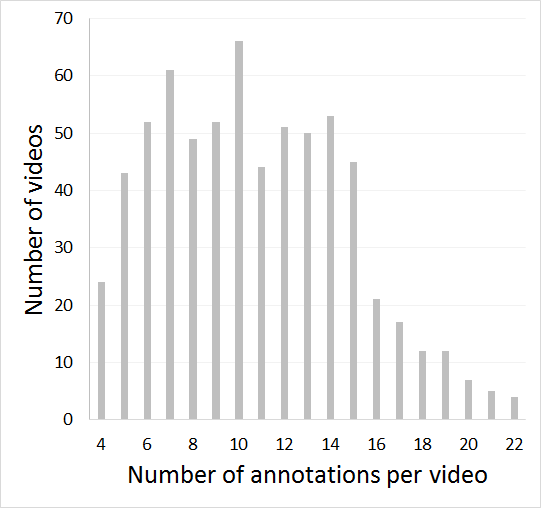
\includegraphics[width=0.3\columnwidth]{figures/histogram_nb_sequences_for_nb_of_annotations.png}}
	\quad
	\subfloat[(b) Human consistency for videos for us]{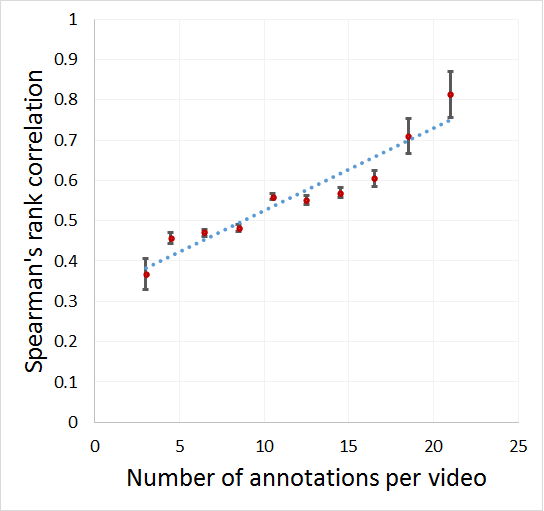
\includegraphics[width=0.3\columnwidth]{figures/Measure_of_human_consistency.png}}
	\caption{\label{fig:human_consistency}(a) Number of sequences for each possible nb of annotations per sequence. (b) Human consistency averaged over 25 random splits (right) obtained using the method proposed by \cite{isola_2014_makes} for sequences with at least 5 annotations (with standard error).}
\end{figure}


%figure Rank corr for Isola et al. et han et al., pour montrer que le nombre d'annotation sva plus vite pour les videos (mais crowdsourcing vs. laboratoire -- et autres facteurs...)

We implemented the method proposed in \cite{isola_2014_makes} to measure the human consistency. It answers the question: "Are the videos that are more memorable (or forgettable) for a group of observers also more likely to be remembered (or forgotten) by a different group of observers? The figure \ref{fig:human_consistency}(b) presents the curve of the human consistency for each video sequence. It answers the question: "How many annotations for each do we need for the human consistency stop varying?'




%compounding factor: most annotated sequences are also the most memorable group, which could artificially increase the Spearman's correlation). 



Individual and contextual differences, besides mandatory random variability, explain the $1-.65$ part of the memorability that is not universally derivable from the intrinsic informations of the videos.  

%Compare our and Khosla et al. curve dire que -- video + non-crowdsourcing + "real" long-term memory -- explique qu'on obtient avec beaucoup moins d'annotation la même human congruency.
If we compare the curve obtained by \cite{khosla_2015_understanding} (\ref{fig:human_consistency}(a))and the curve we obtained (b), we can note than we attain human consistency far more quickly than Khosla \textit{et al.}. At least three arguments go in the way of this results. First, we work with videos and they work with images ; maybe video memorability is more universal than image memorability because of the higher length of this kind of stimulus (but We can also note that the maximum human consistency is close for images and videos!!). Second, we obtain a measure of real long term memorability, and not a memorability measured some minutes after encoding step ; maybe this measure more representative of what is really memorable. Finally, we can advance the fact that in-lab experiment enable to obtain better memorability measure than crowdsourcing one, resulting to attain maximum human consistency earlier.

%%%%%%%%%%%%%%%%%%%%%%%%%%%%%%%%%%%%%
\subsection{Neutral and typical sequences}
% Tester s'il y a une différence entre les deux et en tirer des conséquence quant à leur validité --> How objective our measure of memorability is?

%%%%%%%%%%%%%%%%%%%%%%%%%%%%%%%%%%%%%
\subsection{Quality of the movies}
dvdrip vs. HD 720-1080 => Difference of memorability? => Interesting

%%%%%%%%%%%%%%%%%%%%%%%%%%%%%%%%%%%%%
\subsection{Response time}
Previous authors have integrated response time in their score of memorability. We pose here the following question: "Is the degree of memorability related to response time?" to answer the question: "Should we exploit response time to correct memorability score?" We hypothesized that the most memorable the sequences, the faster the participant will answer (no instructions to answer faster: just to answer durgin the 10-sec display).

%figure Mean response time vs. degrees of memorability
	%with SEM
\begin{figure}[!htbp]
	\centering
	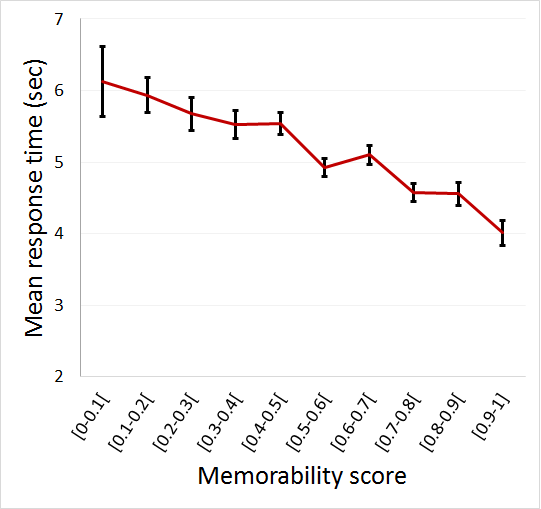
\includegraphics[width=\columnwidth]{figures/Response_time_vs_Memorability.png}
	\caption{\label{fig:response_time_vs_memorability}Mean response time for each memorability degree (error bars correspond to SEM).}
\end{figure}

We observed a Person's correlation of $-0.36 (p<.0001)$ between the response time on the target and their memorability scores. This is consistent with the figure \ref{fig:response_time_vs_memorability}. In other words, the higher the memorability, the lower the response time tends to be, suggesting that a sequence most memorable is also a sequence for which we rapidly detect that it is memorable. This is consistent with what we expected: empirically, we observe during passation that participant tend to answer as soon as they recognized the sequence.

%target vs. fillers
It is interesting to link it to the response time for answer on targets (i.e. correct detections) vs. on fillers (i.e. false alarms). The global mean response time was $4.87 sec$ on targets and $5.96 sec$ on fillers. A Student t-test for different sample size show a significant difference ($t(2836)=-5.34, p<.0001$). This means that the participants globally answered more rapidly for targets (i.e. correct detections) than for fillers (i.e. false alarm). One explanation is that participants hesitated more for fillers they answered on, increasing their response time.

It tells us something on memory, that the memories are not evident but more blurred. This is an important point, taht explained why, in our discussion, we propose to turn to a "totally objective" measure of memory to constitute a dataset for video memorability prediction: if the participants hesitated, so they choice to answer or not was probably impacted by the way they answered the instructions and their own sensibility to the risk.%=> corrigé mémorabilité par individu ?

%How to exploit the response time in the prediction models? --> two potential models for memorabilit prediction


%%%%%%%%%%%%%%%%%%%%%%%%%%%%%%%%%%%%%
\subsection{Evolution of the memorability along time}
%Use order positions for that (e.g. mean memorability for position 1, 2... 120)





%%%%%%%%%%%%%%%%%%%%%%%%%%%%%%%%%%%%%
%tester la mémorability de séquences très proches (prise à intervalles très proche + vérif = même scène)

%indoor/outdorr comme isola et al. mais en contrecarrant l'effet de la couleur -- car ils espliquent que c'est par la corrrélation entre couleur et mémorabilité est expliqué par le fait que les couleurs plus froides sont d'exté.


%%%%%%%%%%%%%%%%%%%%%%%%%%%%%%%%%%%%%
\subsection{New manner to compute memorability scores: take into account time and FA}
%Une nouvelle manière pour prendre en compte les FA dans les scores de mémorabilité applicable à l'étude de la mémorabilité sur les images (si fonction : en parler dan sl'intro comme quoi les gens ne prennent jamais en compte les FA quoiqu'elles puissent être exploiter)
%Ce qui à la fin de cette section vient avant permet de conclure cette partie en disant : la meilleure façon de calculer les scores de mémorabilité, c'est comme ça.



%%%
\subsubsection{Participants' performance}
% The question here is: "Must we correct our memorabiliy scores by taking into account the mean memorability of the participants --> No, of the film --> No' --> So the point here is just to provide an overview.
The average memory performance was the following: the average percentage of correct detection was $48.2\%$ (SD of $14.1\%$) and the average percentage of false alarms was $4.78\%$ (SD of $5.63\%$).


%%%%%%%%%%%%%%%%%%%%%%%%%%%%%%%%%%%%%
\subsection{Logistic regression vs. SVM to personalize prediction model}
%Regression qui prend en compte tous les facteurs (voir ma thèse)
%See QoMEX paper to present the data

%We used the following factors:
	%Occidental/non-occidental, because the 100 movies are occidental (expept slumdog millionaires...)



%%%%%%%%%%%%%%%%%%%%%%%%%%%%%%%%%%%%%
% Other results possible
%%%%%%%%%%%%%%%%%%%%%%%%%%%%%%%%%%%%%
\subsection{Film genre and IMDB ratings}
%test the momorability od the sequences compare to the mean one of the movie.
%Correct bu the mean participant's performance
%And maybe other IMDB annotations/labels

\subsection{Context}
%Analyse the context (order of video presentation) influent the memo: to be check if we have enough information?
%Une vidéo par rapport à toutes les autres différentes à un impact sur sa mem ?
%S'inspirer de la technique de Bylinskii

\subsection{Features linked to memorability}
%tester ces features comme dans 'What makes a photograph...'
% Indoor/Outdoor, low-level visal feautures (color... -- i.e. as in isola et al.), salinecy maps

\subsection{Indoor \textit{.vs} outdoor scenes}



%add other relevant points found in MIT papers e.g.

%%%%%%%%%%%%%%%%%%%%%%%%%%%%%%%%%%%%%
\subsection{Memorability score calculation}
According to what was presented before in tis section, this is how we finally decided to compute our memorability scores...

%quality of the movies: dvdrip vs. HD 720-1080 => Difference of memorability? => Interesting


%%%%%%%%%%%%%%%%%%%%%%%%%%%%%%%%%%%%%%%%%%%%%%%%%%%%%%%%%%%%%%%%%%%%%%%%%%%%%%%%%%%%%%%%%%%%%%%%%%%%%%%%%%%%%%%%%%%%%%%%%%%%%%%%%%%%%%%%%%%%%%%%%%%%%%%%%
\section{MEMORABILITY PREDICTION} %for Khartik
%%%%%%%%%%%%%%%%%%%%%%%%%%%%%%%%%%%%%%%%%%%%%%%%%%%%%%%%%%%%%%%%%%%%%%%%%%%%%%%%%%%%%%%%%%%%%%%%%%%%%%%%%%%%%%%%%%%%%%%%%%%%%%%%%%%%%%%%%%%%%%%%%%%%%%%%%











%%%%%%%%%%%%%%%%%%%%%%%%%%%%%%%%%%%%%%%%%%%%%%%%%%%%%%%%%%%%%%%%%%%%%%%%%%%%%%%%%%%%%%%%%%%%%%%%%%%%%%%%%%%%%%%%%%%%%%%%%%%%%%%%%%%%%%%%%%%%%%%%%%%%%%%%%
\section{CONCLUSIONS AND FUTURE WORKS}
%%%%%%%%%%%%%%%%%%%%%%%%%%%%%%%%%%%%%%%%%%%%%%%%%%%%%%%%%%%%%%%%%%%%%%%%%%%%%%%%%%%%%%%%%%%%%%%%%%%%%%%%%%%%%%%%%%%%%%%%%%%%%%%%%%%%%%%%%%%%%%%%%%%%%%%%%
% Nous construisons actuellement une base de données de grande ampleur avec une mesure purement objective de la mémoire.
%Nulle part les auteurs ne parlent de mémoire à long terme, à court terme… => Ils appréhendent un problème par nature interdisciplinaire d’un point de vue purement computer science => Or la qualité des données est ce qui détermine ce que les modèles vont finalement prédire. // %D'abord, le test de mémoire interroge une mémoire de vidéos vues longtemps (en moyenne, probablement plusieurs mois ou années) auparavant.
%cite QooMEX for personlization of memorability model

% A conclusion section is not required. Although a conclusion may review the main points of the paper, do not replicate the abstract as the conclusion. A conclusion might elaborate on the importance of the work or suggest applications and extensions. 

%%%
 %Liste des features (comme/ceux de MediaEval 2015 à donner au téléchargement avec le début en sec de nos sequences)
 %Release text file for movie title, start/end time + features

%file to make the data + movies names available.

%In particular, our protocol try to correct to integrate the concept of "very long-term memory", that escaped to previous studie in image and videos, which measured the memory of items some minutes after the memory encoding.


%anntation des séquences pas à même vitesse, en cas de généralisation : changer les séquences annoté plus de 15 fois par exemple par de nouvelles.


% Conclusion => Nos travaux futurs





\addtolength{\textheight}{-12cm}   % This command serves to balance the column lengths
                                  % on the last page of the document manually. It shortens
                                  % the textheight of the last page by a suitable amount.
                                  % This command does not take effect until the next page
                                  % so it should come on the page before the last. Make
                                  % sure that you do not shorten the textheight too much.


%%%%%%%%%%%%%%%%%%%%%%%%%%%%%%%%%%%%%%%%%%%%%%%%%%%%%%%%%%%%%%%%%%%%%%%%%%%%%%%%%%%%%%%%%%%%%%%%%%%%%%%%%%%%%%%%%%%%%%%%%%%%%%%%%%%%%%%%%%%%%%%%%%%%%%%%%
\section*{APPENDIX}
%%%%%%%%%%%%%%%%%%%%%%%%%%%%%%%%%%%%%%%%%%%%%%%%%%%%%%%%%%%%%%%%%%%%%%%%%%%%%%%%%%%%%%%%%%%%%%%%%%%%%%%%%%%%%%%%%%%%%%%%%%%%%%%%%%%%%%%%%%%%%%%%%%%%%%%%%
%Appendixes should appear before the acknowledgment.

%%%%%%%%%%%%%%%%%%%%%%%%%%%%%%%%%%%%%%%%%%%%%%%%%%%%%%%%%%%%%%%%%%%%%%%%%%%%%%%%%%%%%%%%%%%%%%%%%%%%%%%%%%%%%%%%%%%%%%%%%%%%%%%%%%%%%%%%%%%%%%%%%%%%%%%%%
\section*{ACKNOWLEDGMENT}
%%%%%%%%%%%%%%%%%%%%%%%%%%%%%%%%%%%%%%%%%%%%%%%%%%%%%%%%%%%%%%%%%%%%%%%%%%%%%%%%%%%%%%%%%%%%%%%%%%%%%%%%%%%%%%%%%%%%%%%%%%%%%%%%%%%%%%%%%%%%%%%%%%%%%%%%%
%This section is optional; it is a location for you
%to acknowledge grants, funding, editing assistance and
%what have you.

%%%%%%%%%%%%%%%%%%%%%%%%%%%%%%%%%%%%%%%%%%%%%%%%%%%%%%%%%%%%%%%%%%%%%%%%%%%%%%%%%%%%%%%%%%%%%%%%%%%%%%%%%%%%%%%%%%%%%%%%%%%%%%%%%%%%%%%%%%%%%%%%%%%%%%%%%
%% BIBLIOGRAPHY
%%%%%%%%%%%%%%%%%%%%%%%%%%%%%%%%%%%%%%%%%%%%%%%%%%%%%%%%%%%%%%%%%%%%%%%%%%%%%%%%%%%%%%%%%%%%%%%%%%%%%%%%%%%%%%%%%%%%%%%%%%%%%%%%%%%%%%%%%%%%%%%%%%%%%%%%%
\bibliographystyle{ACM-Reference-Format}
\bibliography{references} 

%%%%%%%%%%%%%%%%%%%%%%%%%%%%%%%%%%%%%%%%%%%%%%%%%%%%%%%%%%%%%%%%%%%%%%%%%%%%%%%%%%%%%%%%%%%%%%%%%%%%%%%%%%%%%%%%%%%%%%%%%%%%%%%%%%%%%%%%%%%%%%%%%%%%%%%%%
\end{document}